\documentclass{beamer}
\usetheme{default}
\setcounter{tocdepth}{2} % Set the depth of table of contents to include subsections
%\setbeamertemplate{footline}[frame number]


\setbeamertemplate{footline}{
  \leavevmode%
  \hbox{%
  \begin{beamercolorbox}[wd=.9\paperwidth,ht=2.25ex,dp=1ex,leftskip=3ex,rightskip=3ex]{author in head/foot}%
    \usebeamerfont{author in head/foot}\insertshortauthor\hfill\insertshorttitle
  \end{beamercolorbox}%
  \begin{beamercolorbox}[wd=.1\paperwidth,ht=2.25ex,dp=1ex,right]{author in head/foot}%
    \usebeamerfont{author in head/foot}\insertframenumber{} / \inserttotalframenumber
  \end{beamercolorbox}}%
  \vskip0pt%
}

\usepackage{tikz}
\usepackage{emoji}
\usepackage{fontawesome5}

\title{Mastering Multitenant Orchestration with dbt and Dagster}
\subtitle{Life of Data Engineers does not have to be that hard}
\author{Andrea Montes}
\date{\the\year{}-0\the\month{}}
\institute{DBT Bogotá Meetup}

\begin{document}

\begin{frame}
    \titlepage
\end{frame}

\begin{frame}
    \tableofcontents
\end{frame}

\section{Audience questions}
\begin{frame}
    \frametitle{Audience questions}
    \begin{enumerate}
        \item Airflow familiarity?
        \item Crazy tools difficult to debug?
    \end{enumerate}
\end{frame}

\section{Problem}
\begin{frame}
    \frametitle{What is needed?}
    \begin{itemize}
        \item Daily updates to client dashboards. +250 different clients
        \item Custom reports per client
        \item Product and business questions
    \end{itemize}
\end{frame}

\begin{frame}
    \frametitle{Legacy product(s) - Data Warehouse}
    \begin{figure}
        \centering
        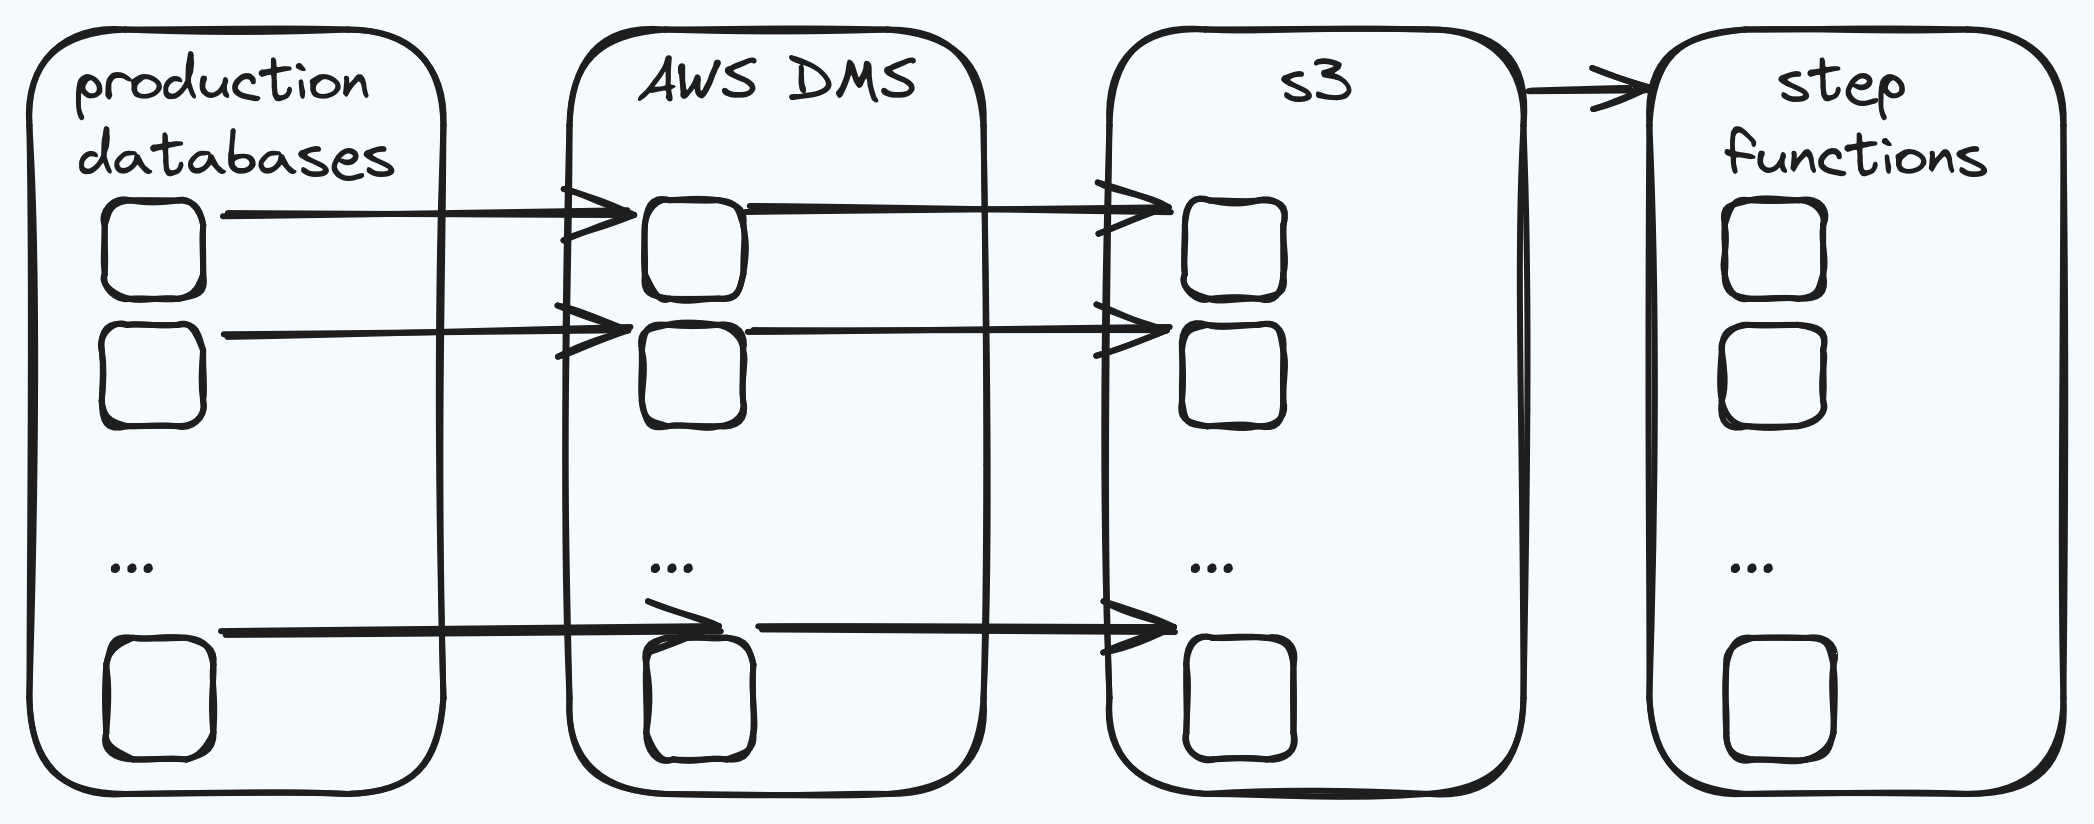
\includegraphics[width=1\textwidth]{pictures/legacy_product}
        \caption{Legacy DWH product}
    \end{figure}
    \begin{itemize}
        \item Daily refresh
        \item Failed 2 or 4 times a week for heavy clients \emoji{weary}
    \end{itemize}
    \end{frame}

\begin{frame}
\frametitle{Legacy product(s) - Reporting}
    \begin{figure}
        \centering
        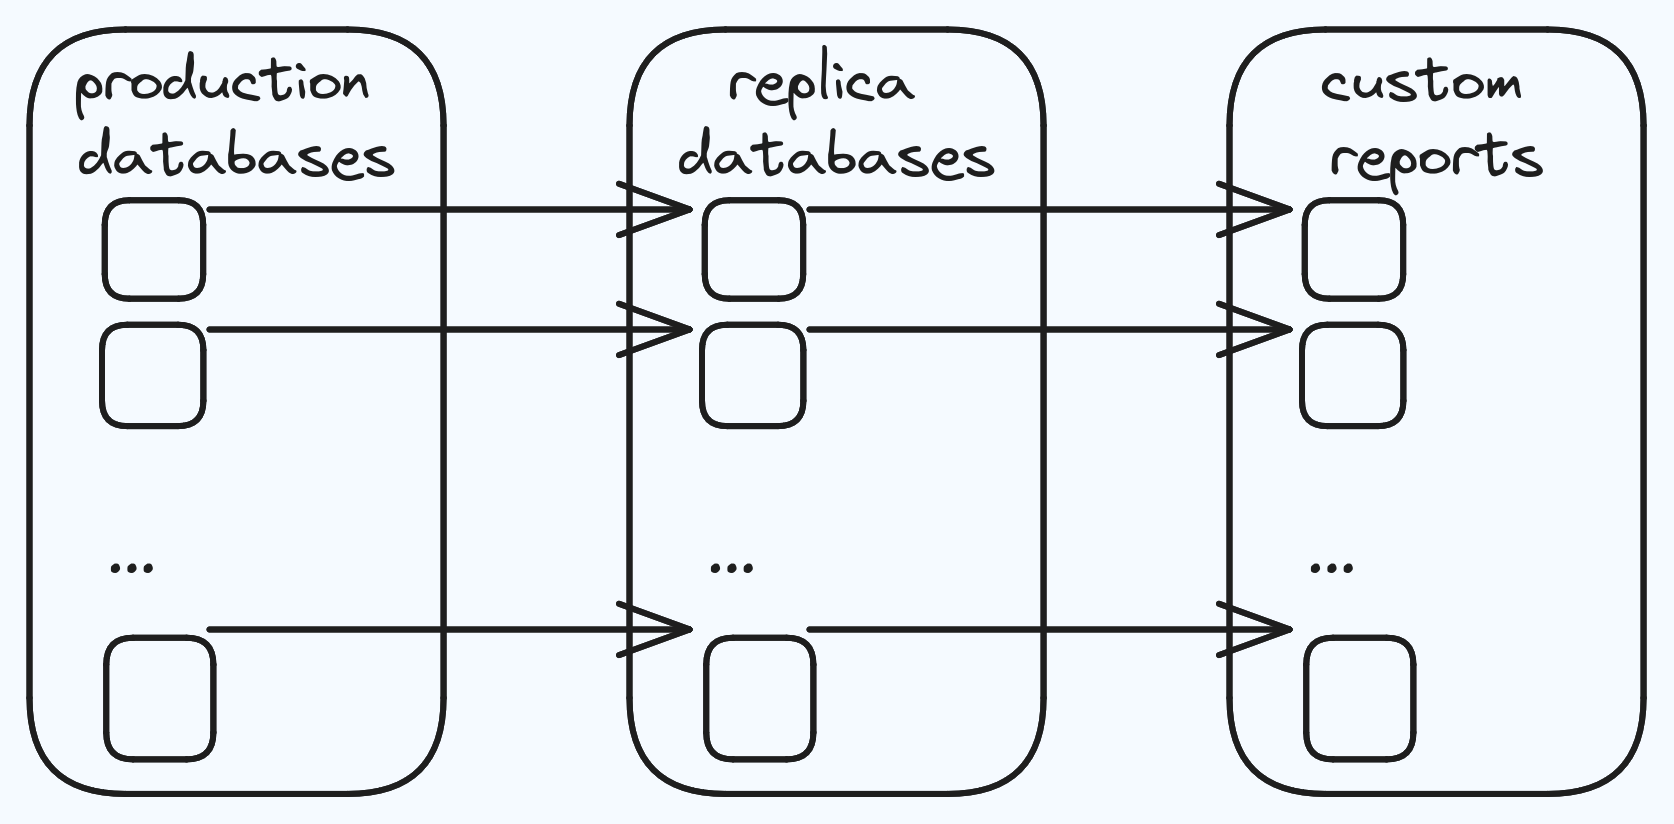
\includegraphics[width=1\textwidth]{pictures/legacy_reporting}
        \caption{Legacy reporting product}
    \end{figure}
    \begin{itemize}
        \item Replicated once a week \emoji{expressionless}
        \item Raw sql
        \item Stored procedures
    \end{itemize}
\end{frame}

\section{We need to re-design}
\begin{frame}
\frametitle{We need to re-design}
\end{frame}

\subsection{Requirements}
\begin{frame}
    \frametitle{Different users, different requirements}

    \begin{block}{Dashboards}
        Clients need their dashboards updated to know events statuses
    \end{block}

    \begin{alertblock}{Business questions}
        What are the most used features?, how virtual vs in-person events attendance has changed after pandemic \emoji{mask}?
    \end{alertblock}

    \begin{exampleblock}{Client questions}
        How long is taking a candidate to become an applicant? Do I have a diverse pipeline?
    \end{exampleblock}
\end{frame}

\subsection{New architecture}

\begin{frame}
    \frametitle{New architecture}
    \begin{figure}
        \centering
        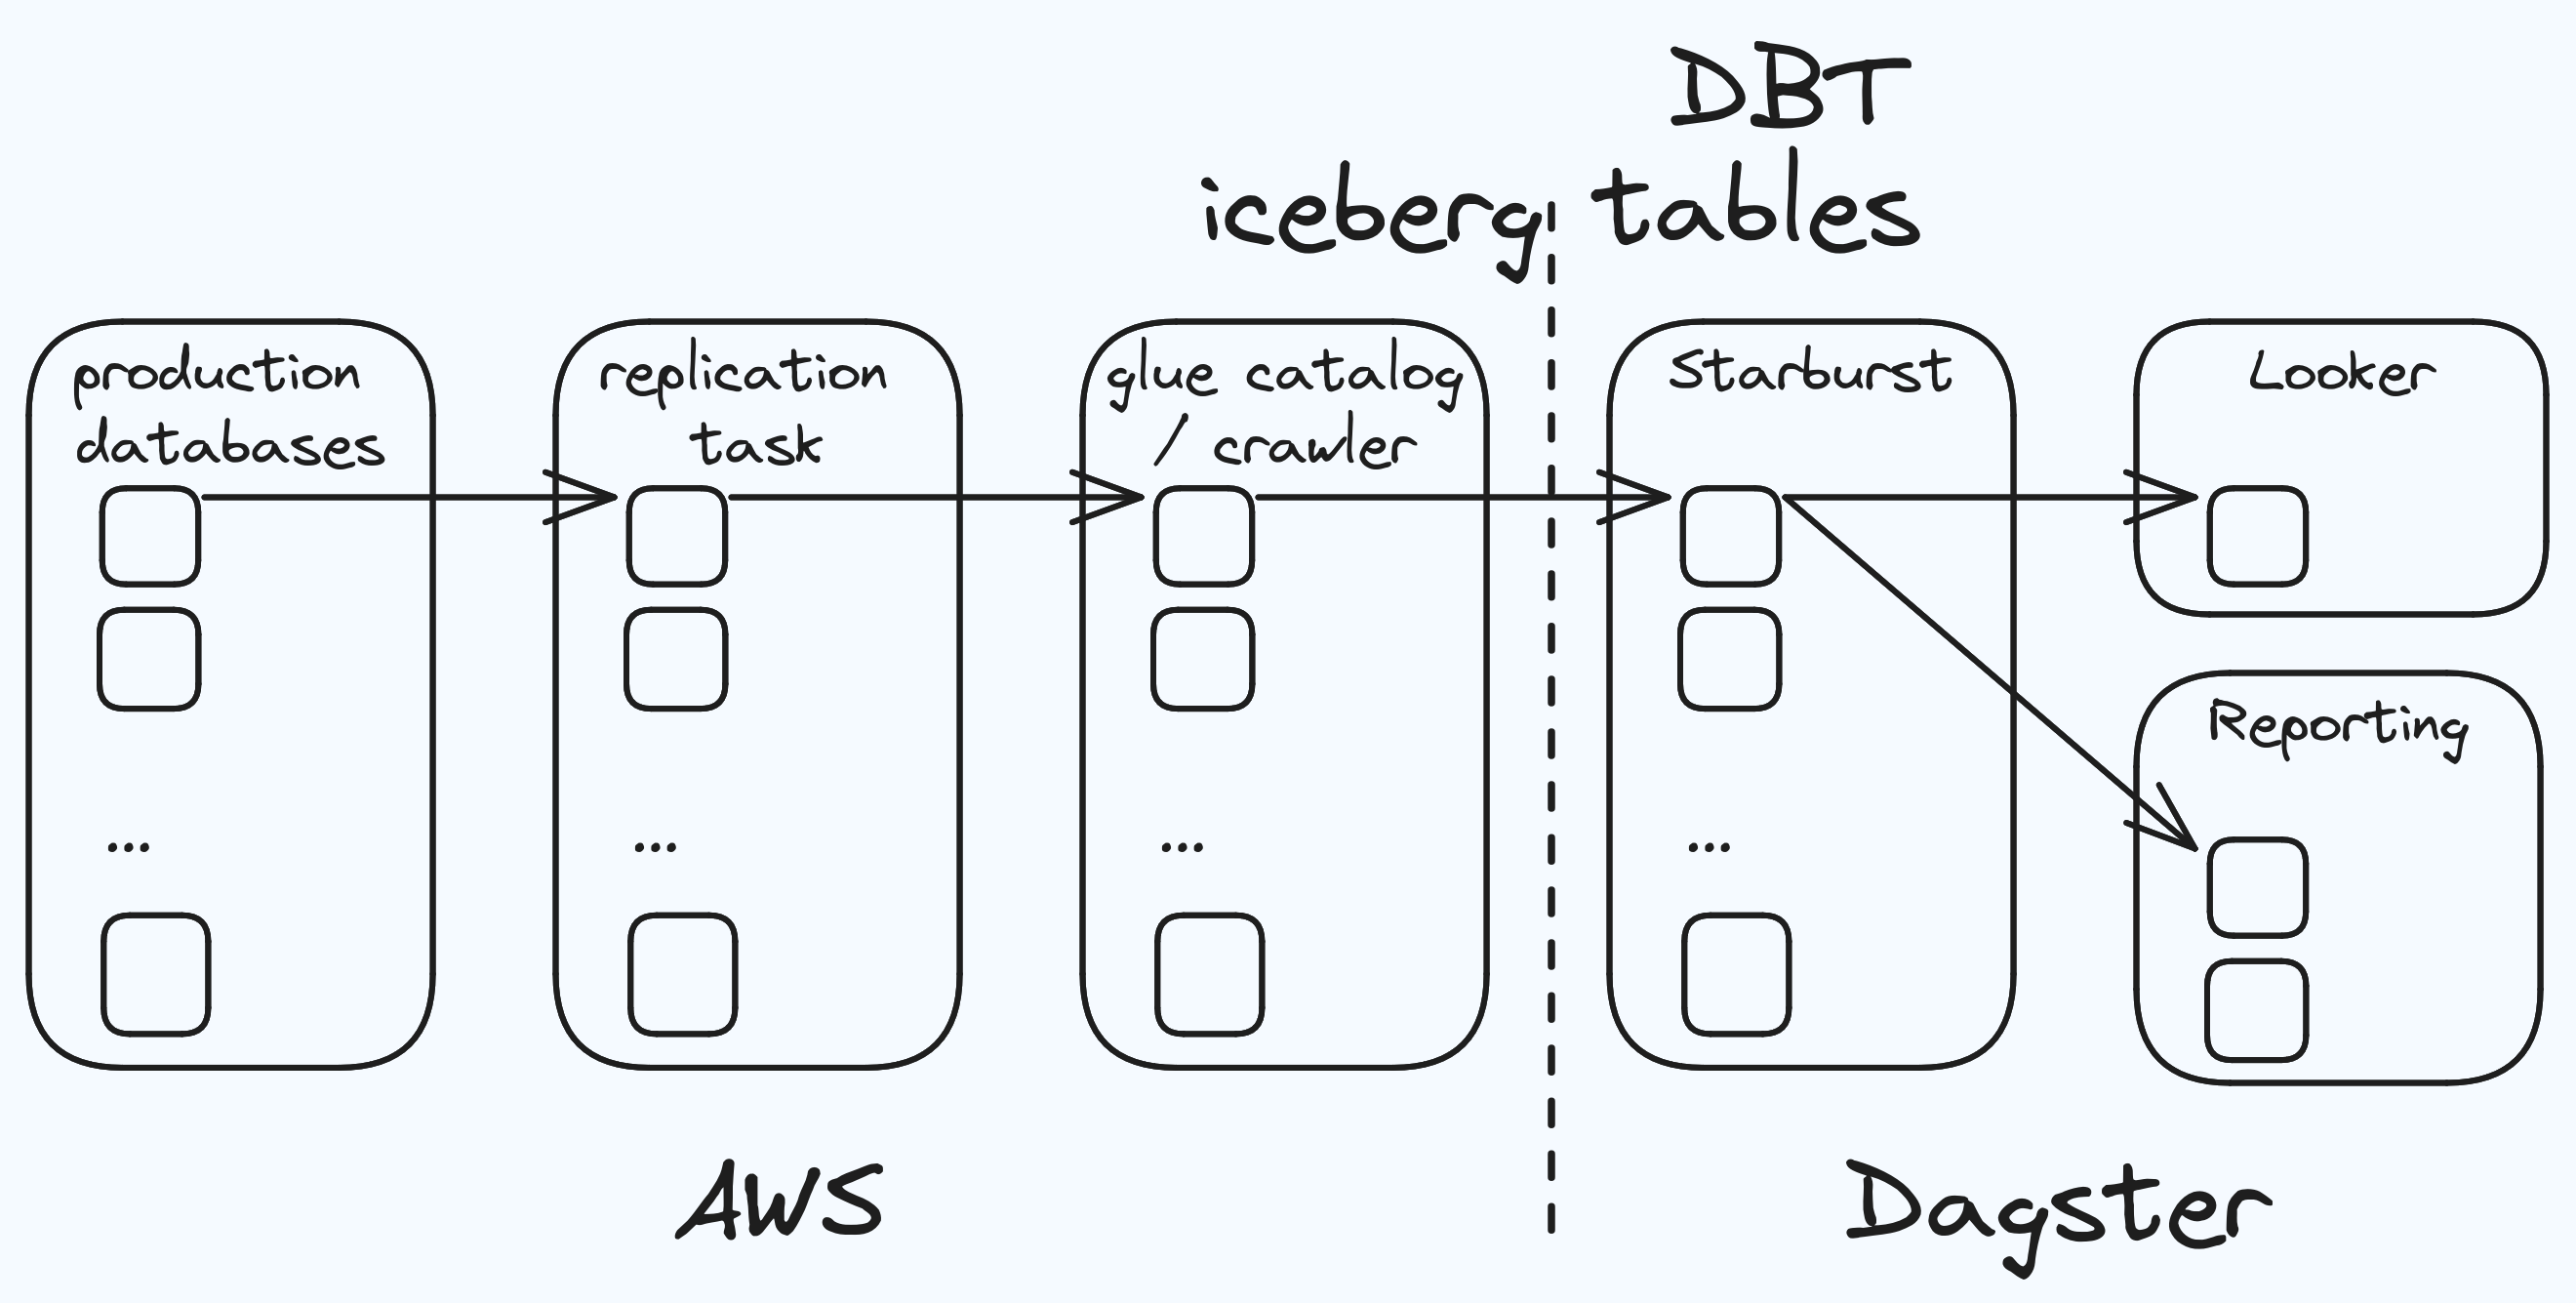
\includegraphics[width=1\textwidth]{pictures/architecture}
        \caption{New architecture to accomplish reporting and DWH requirements}
    \end{figure}
\end{frame}

\subsection{Stage: Extract}
\begin{frame}
    \frametitle{DMS}
    \begin{itemize}
        \item Cheap...
        \item Not reliable as we would like
        \item Trade-off
    \end{itemize}
\end{frame}

\subsection{Stage: Load}
\begin{frame}
    \frametitle{Glue catalog and Crawler}
    \begin{itemize}
        \item Easy enough to implement
        \item Our compute engine support it
    \end{itemize}
\end{frame}

\subsection{Stage: Transformation}
\begin{frame}
    \frametitle{Starburst - DBT}
    \begin{columns}
        \begin{column}{0.5\textwidth}
            \emoji{thumbs-up}
            \begin{itemize}
                \item Starburst is a vendor option for Trino
                \item Cheaper than snowflake
                \item Trino has a good community
            \end{itemize}
        \end{column}
        \begin{column}{0.5\textwidth}
            \emoji{thumbs-down}
            \begin{itemize}
                \item SQL ANSI
                \item It's a new product, random changes
                \item Compute throttling
                \item We were their first large user
            \end{itemize}
        \end{column}
    \end{columns}
\end{frame}

\subsection{Stage: Transformation - Leveraging DBT for multitenancy}

\begin{frame}
    \frametitle{DBT and multiple clients}
    \begin{columns}
    \begin{column}}{0.5\textwidth}
        \begin{verbatim}
        SELECT
            AÑO AS year
            , TRIMESTER AS trimester
            , PROVEEDOR AS provider
            , "LINEAS EN SERVICIO" AS lines_in_service
            , "LINEAS PREPAGO" AS prepaid_lines
            , "LINEAS POSPAGO" AS postpaid_lines
            , "LINEAS ACTIVADAS" AS enabled_lines
            , "LINEAS RETIRADAS" AS retired_lines
        FROM {{ ref('mobile_phone_subscribers_by_category')}}
        WHERE PROVEEDOR = '{{ var("client")}}'
        \end{verbatim}
    \end{column}
    \begin{column}}{0.5\textwidth}

    \end{column}
    \end{columns}
\end{frame}

\begin{frame}
    \frametitle{DBT and multiple clients}
    \begin{figure}
        \centering
        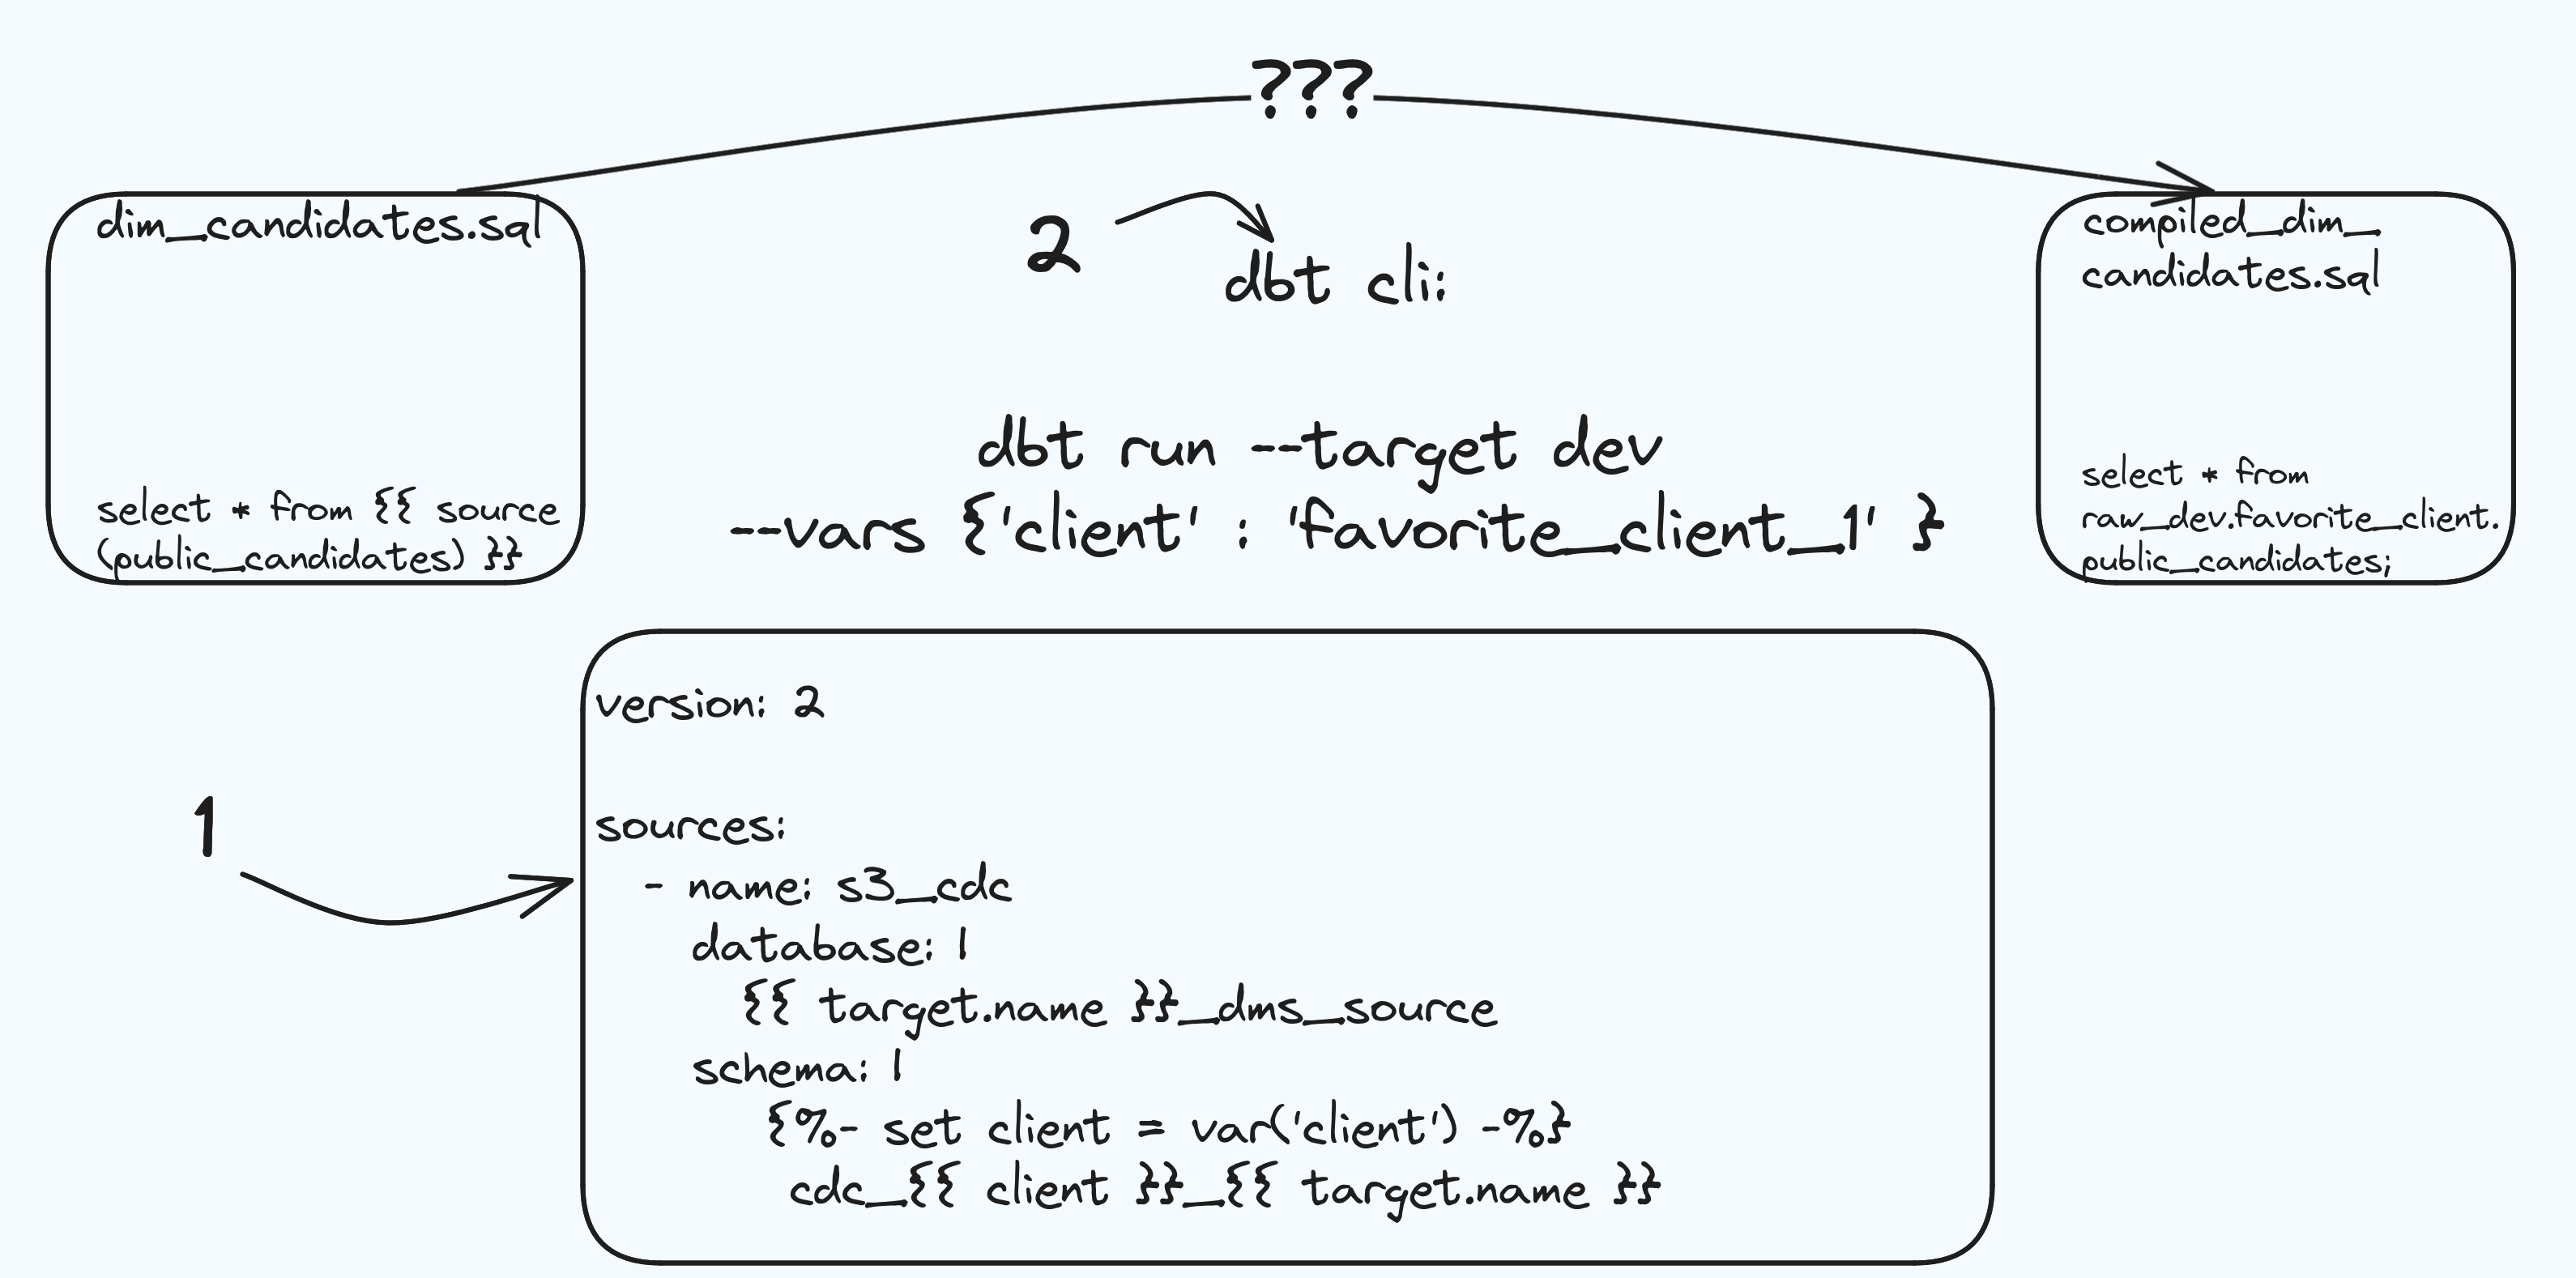
\includegraphics[width=1\textwidth]{pictures/multitenancy_dbt}
        \caption{Multitenancy sorted out using dbt cli and variables}
    \end{figure}
\end{frame}

\subsection{Stage: Transformation - but for +250 clients?}
\begin{frame}
    \frametitle{Orchestration tool: Dagster}
    \begin{columns}
        \begin{column}{0.5\textwidth}
            \begin{figure}
                \centering
                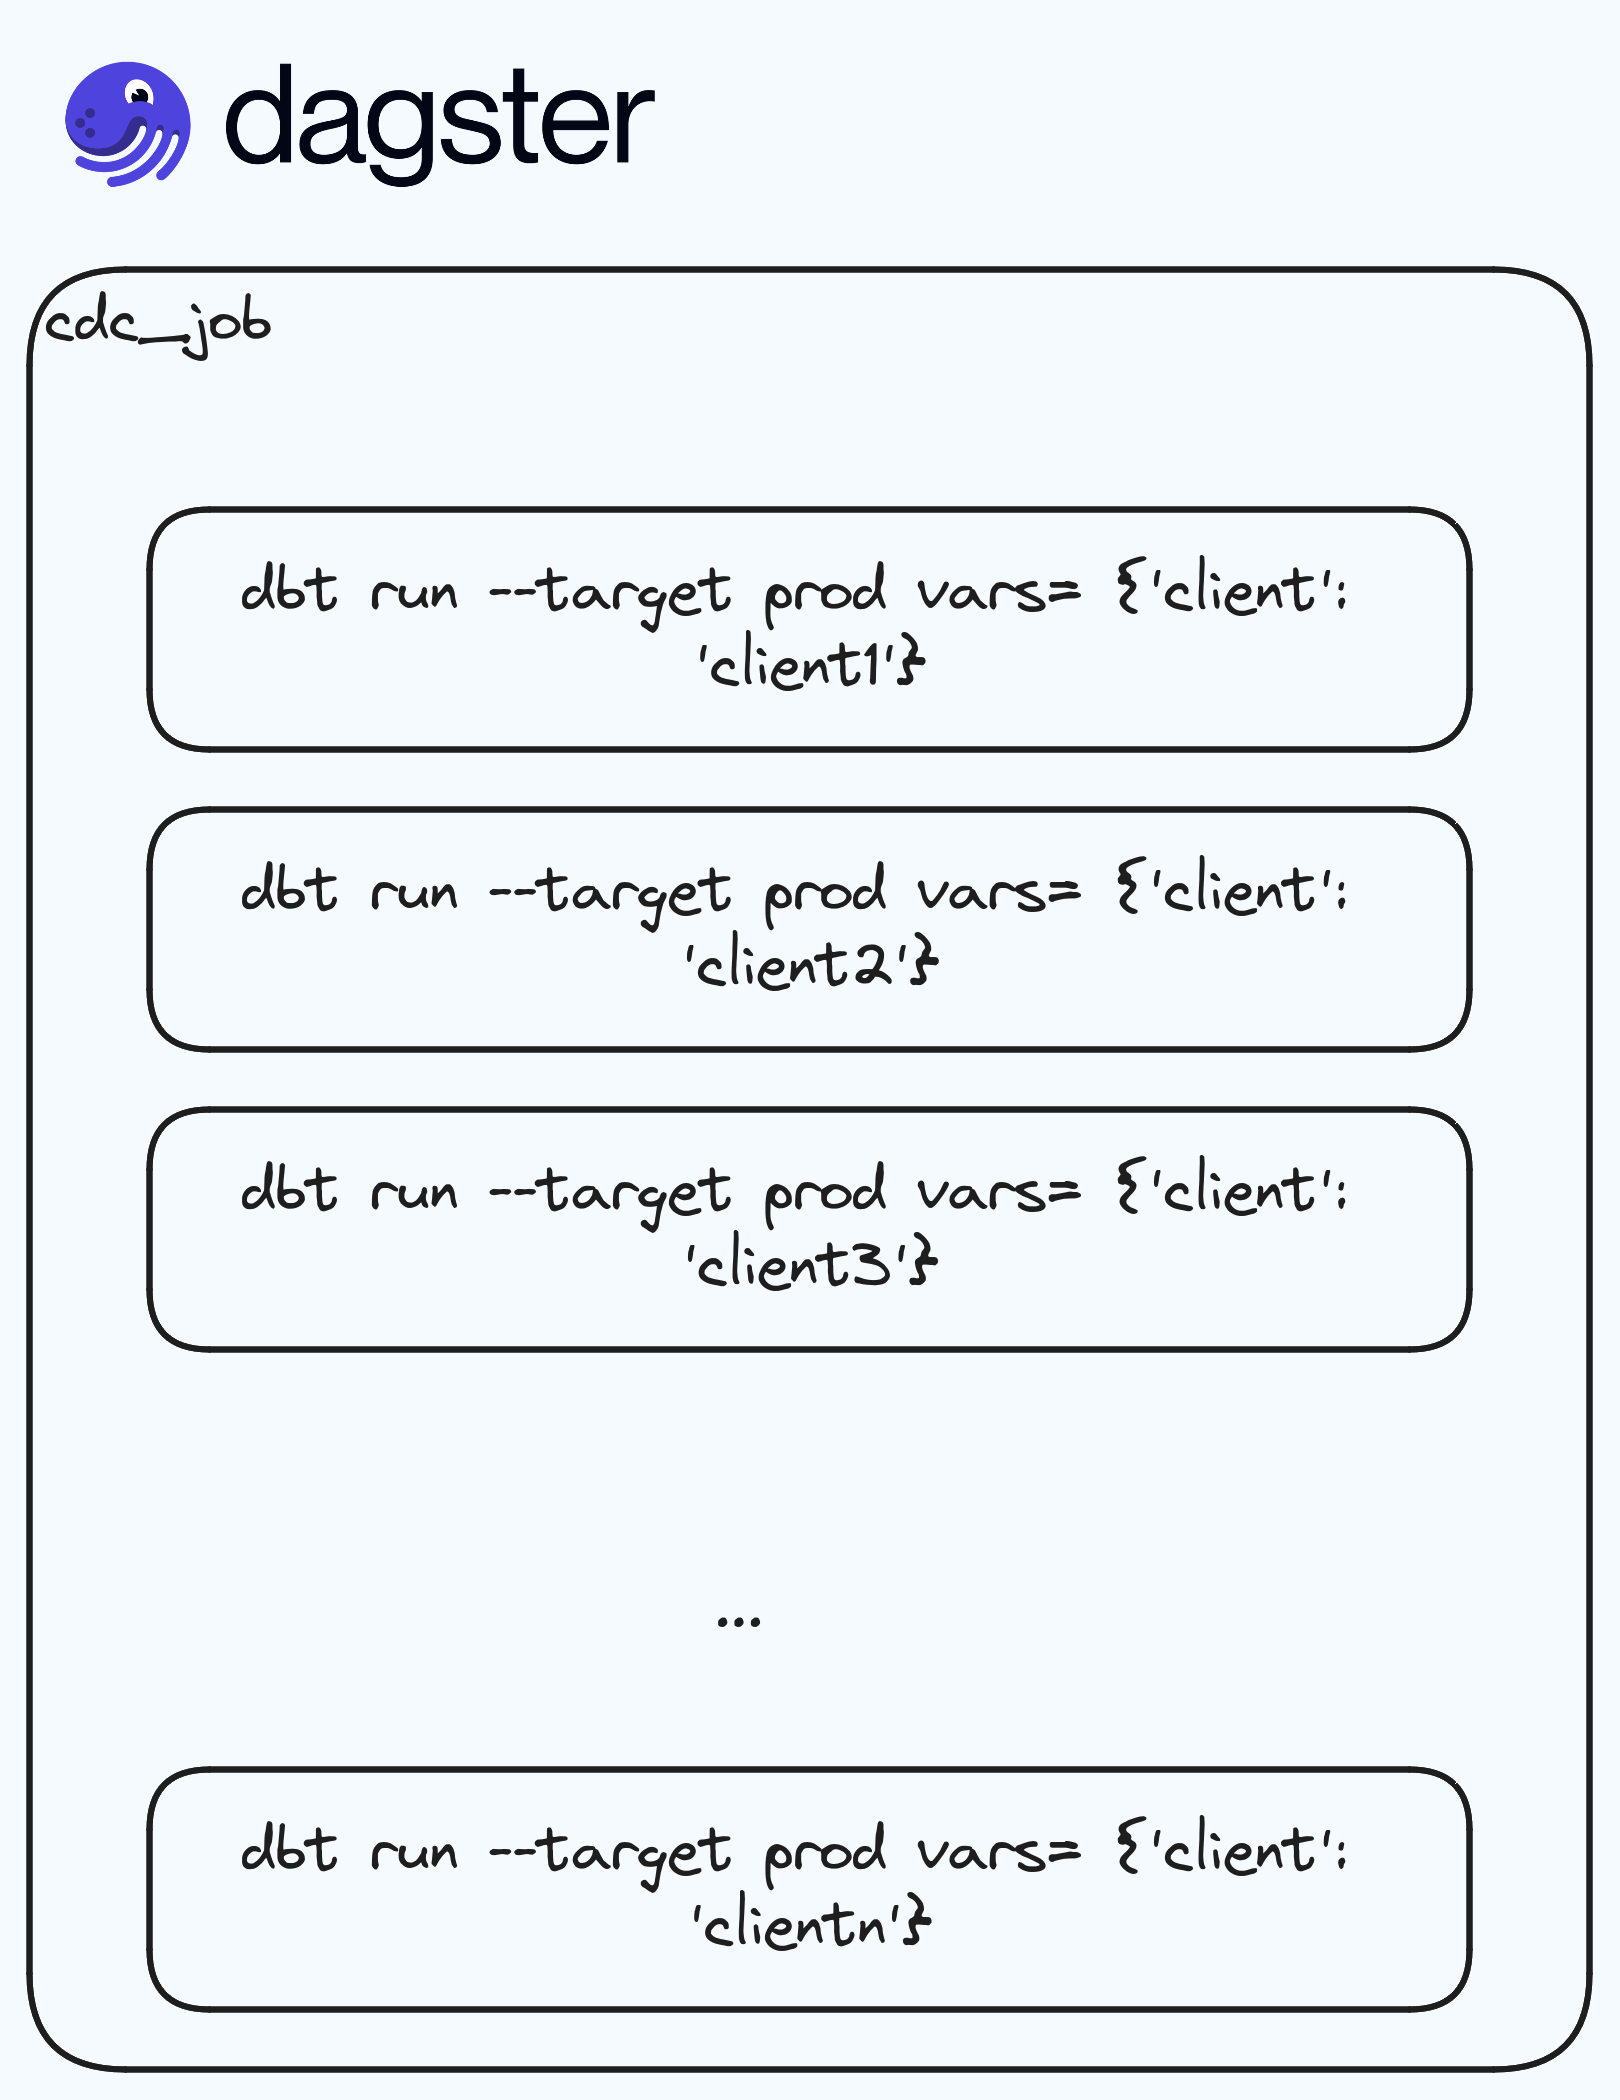
\includegraphics[width=1\textwidth]{pictures/dagster_job}
                \caption{Dagster: How do we run 250 dbt commands?}
            \end{figure}
        \end{column}
        \begin{column}{0.5\textwidth}
            \begin{itemize}
                \item We run cdc\_job daily starting at 2 am CST
                \item Each job client partition takes about 7 mins
                \item Job finishes before 7 am CST
            \end{itemize}
        \end{column}
    \end{columns}
\end{frame}


\section {Takeaways}
\begin{frame}
    \frametitle{Takeaways}
    \begin{itemize}
        \item Not getting used to what is poorly done
        \item Don't fall in love with a technology product
    \end{itemize}
\end{frame}

\begin{frame}
    \frametitle{Who am I?}
    \begin{columns}
        \begin{column}{0.5\textwidth}
        \begin{figure}
            \begin{tikzpicture}
                \clip (0,0)  circle (2cm) ;
                \node[anchor=center] at (0,0) {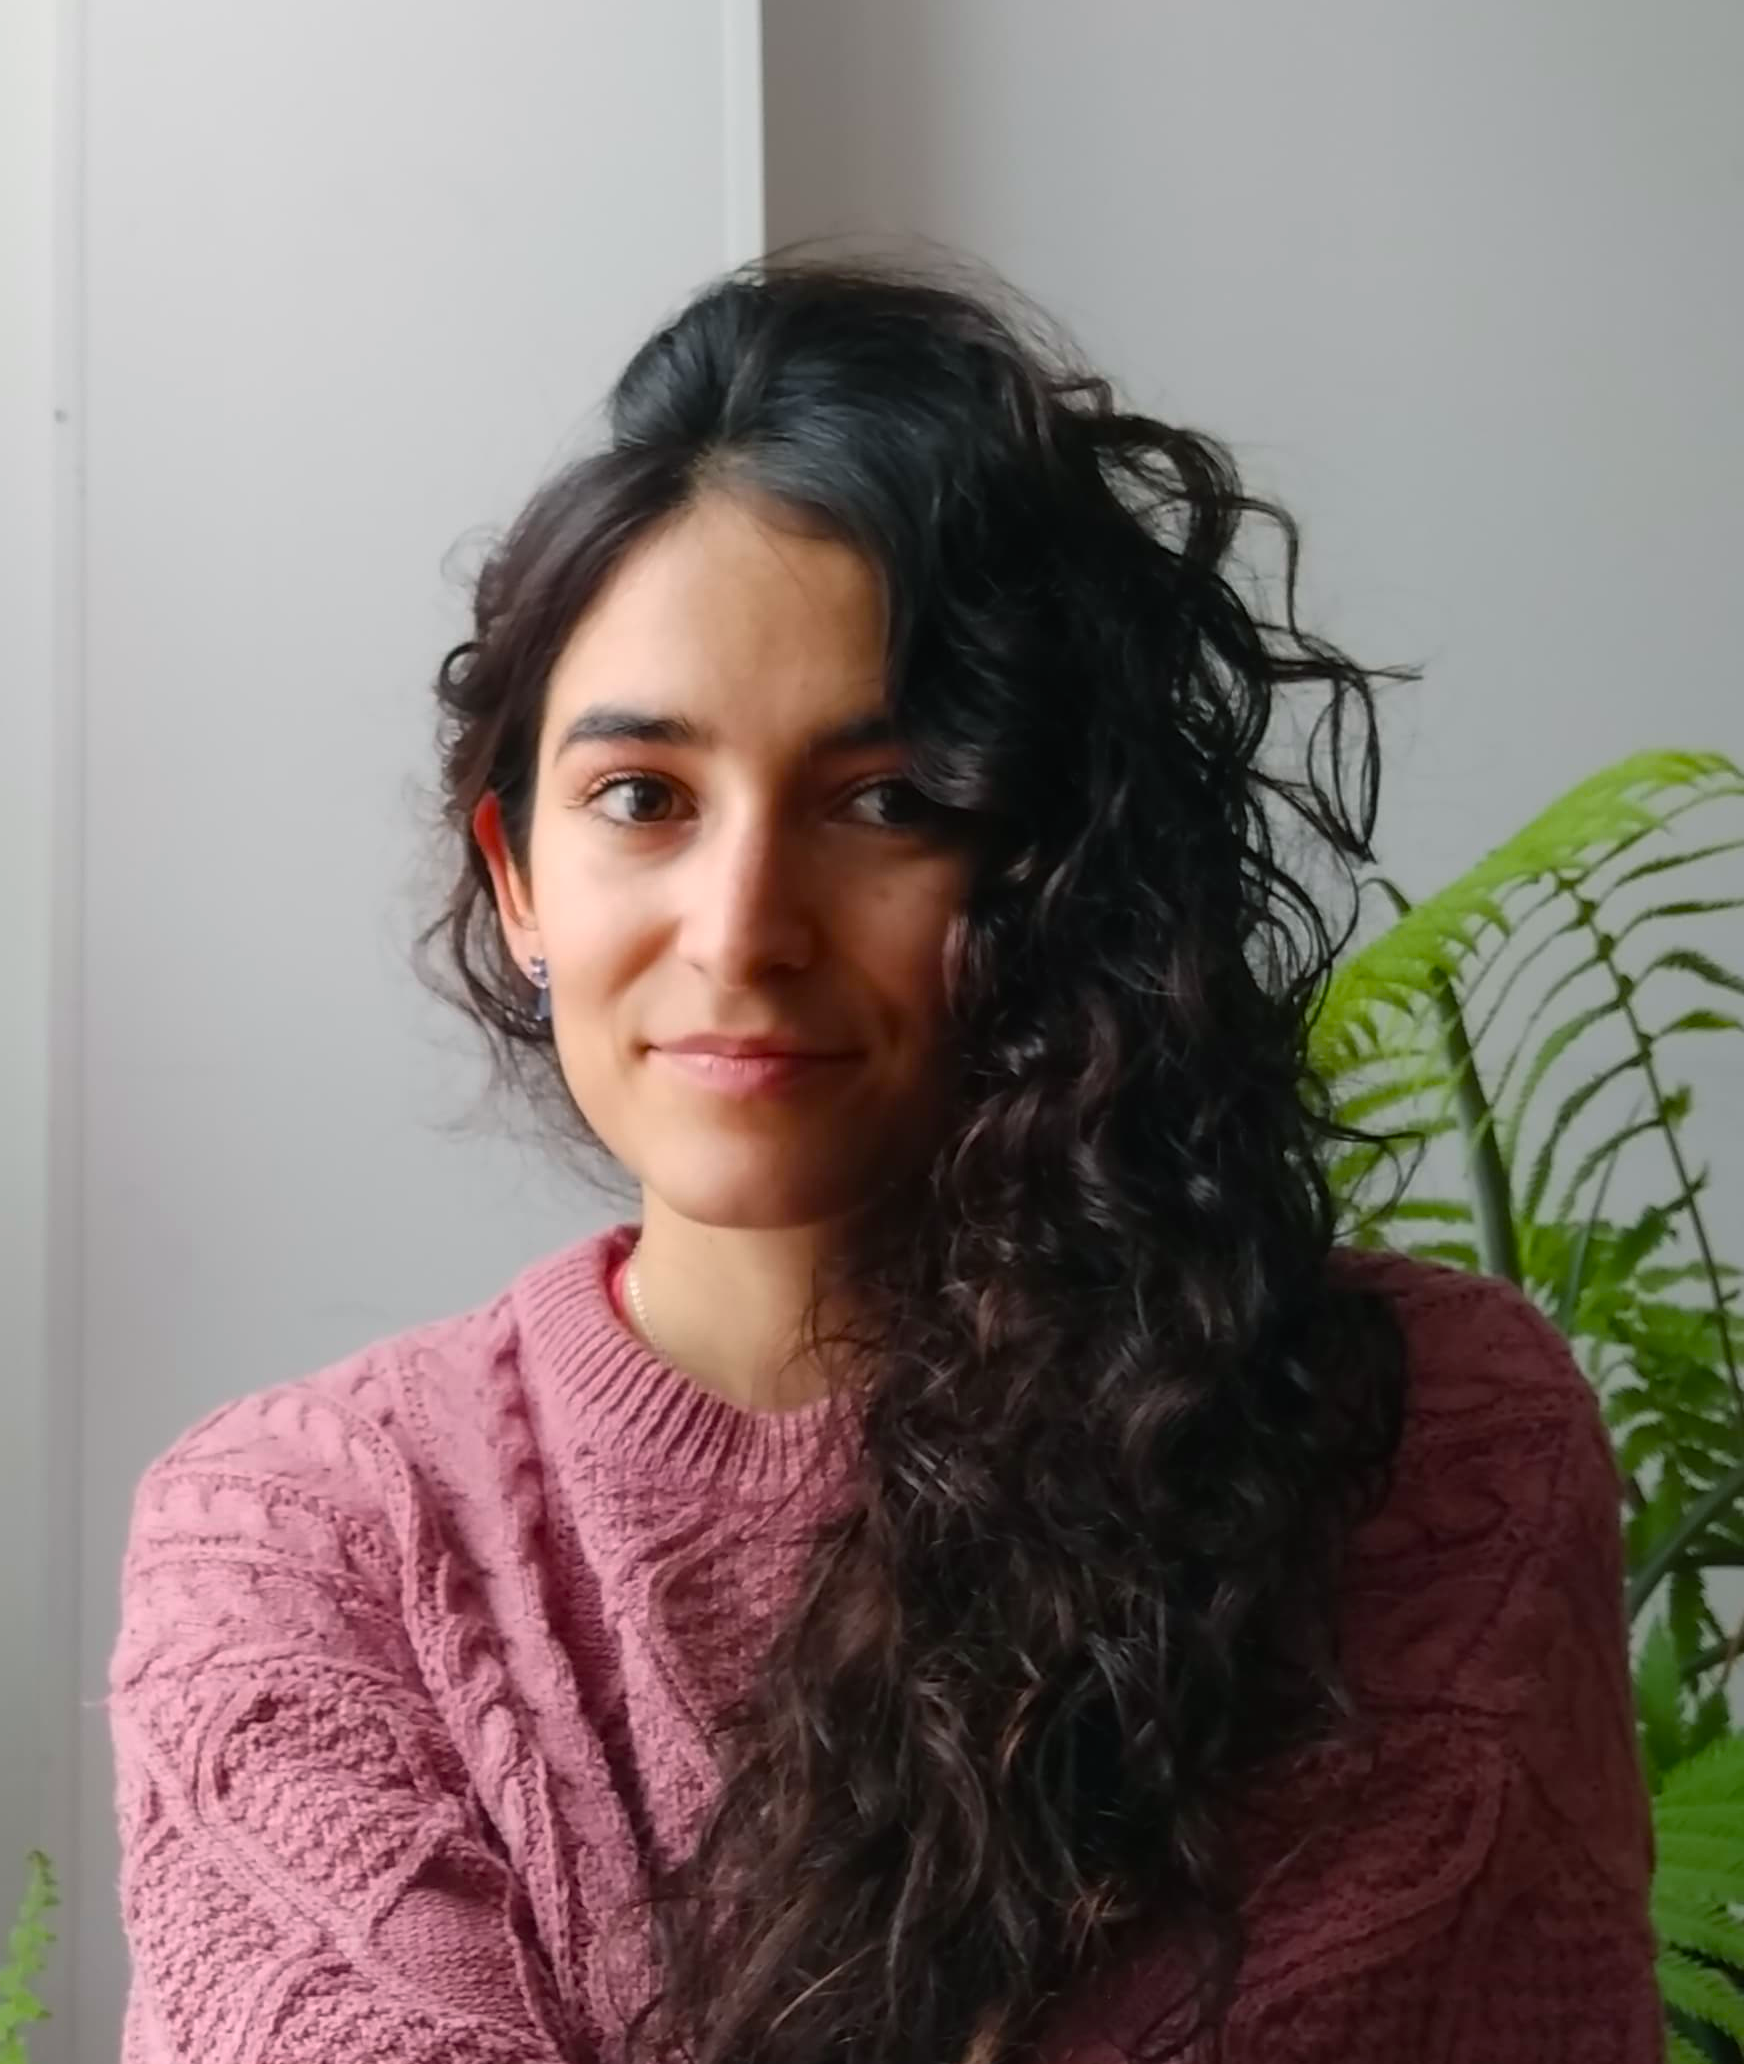
\includegraphics[width=0.8\textwidth]{pictures/me}};
                %adjust this coordinate to move image
            \end{tikzpicture}
        \caption{Andrea Montes}
        \end{figure}
        \end{column}

        \begin{column}{0.5\textwidth}
         \href{https://www.linkedin.com/in/mamontesp}{\faLinkedin \ Andrea Montes - Senior Data Engineer}
         
         \smallskip
         
         \href{https://github.com/mamontesp}{\faGithub \ mamontesp}

        \end{column}
    \end{columns}
\end{frame}
\end{document}